\chapter{MSN models (Medium-spiny neurons)}
\label{chap:MSN-models}

Sect.\ref{sec:medium_spiny_neurons} introduces MSN neurons.

\section{Electrophysiological properties}

The whole cell K + current recorded from neostriatal
cells is composed of three components:
\begin{enumerate}
  \item fast-inactivating A current (KAf): Kv4.x; sensitive to 4-AP (i.e.
  blocked by relatively high, IEC50 = 2mM 4-AP)
  
 activate quickly at or above the spike threshold, then inactivate quickly
 within 50-100 ms. 
  
  
  \item slowly inactivating A current (KAs): sensitive to 4-AP (i.e. blocked by
  low concentration of 4-AP, IC50 = 100$\muM$)
  
 activate quickly at subthreshold membrane potentials, inactivates over 
 hundreds of miliseconds
  
  \item delayed-rectifier, persistent component 
\end{enumerate}

Nisenbaum et al. (1996) - whole-cell recording K+ currents: usually < 500 pA
(and no more than 1 nA) (check Sect.\ref{sec:MSN-morphology} for somatic surface
area).

\subsection{resting potential (down-state)}


\textcolor{red}{\bf Kir2.x}:
MSN exhibit a highly polarized resting membrane potential:
$V_\rest \approx -80 $mV (a 'down-state'), where Kir2 dominate the conductance
profile (Sect.\ref{sec:Kir2.x})
\begin{itemize}
  \item  mean resting membrane potential of -87.75 mV in MSN of NAc [Wolf et
  al., 2005]
\end{itemize}

\subsection{up-state}

\textcolor{red}{\bf Kv4.x}: Upon synaptically driven depolarization, the MSN can
move from 'down-state' to a depolarized 'up-state' (ca. -60 mV) near the
threshold, in response to temporal coherent glutamatergic inputs. In parallel,
is the reducing of inward current from Kir2.x. However, the depolarization then
faces a barrier of an outward current, i.e. which is quickly activate in the
given voltage range and is composed of Kv4 family subunits
(Sect.\ref{sec:Kv4-channels}).

\textcolor{red}{\bf Kv1}:
Kv4 activate early during depolarization, but also inactivate relatively
rapidly, making them poor regulators of sustained depolarizing inputs as seen in
'up-state'. This role is played by another K+ channel which open at a
subthreshold voltage range but unlike Kv4 channels inactivates slowly, which
resemble what has been referred to as the D-type current (Storm 1988) or the
slowly inactivating A-type current (Albert and Nerbonne 1995; Locke and Nerbonne
1997; Surmeier et al. 1991). This current slows the subthreshold ramp potential
induced by depolarizing current injection and slows repetitive spike rate.
\begin{itemize}

  \item until 2003: the molecular identity (or identities) of this slowly inactivating
 K+ channel in medium spiny neurons has yet to be determined.

The biophysical and pharmacological data gathered to date point to a Kv1 family
channel (Sect.\ref{sec:Kv1-channels}) and based on data at somatic and proximal
dendrites in rat striatum, it was confirmed as Kv1.2 subunits [Shen- Surmeier,
2003].
In the subthreshold voltage range, this Kv1.2 channel current constitutes nearly
half of the total somatic K+ current, leading to a major role in regulating
spike threshold and repetitive discharge.

% based on (1) the slowly inactivating
% current is sensitive to 4-aminopyridine (4-AP) at micromolar concentrations and
% to $\alpha$-dendrotoxin ($\alpha$-DTX) (Nisenbaum et al. 1994, 1996); (2)
% recovery from inactivation is slow, e.g. greater than a second at -90 mV
% (Surmeier et al. 1991).



\end{itemize}

There are also 4-AP sensitive K+ current (Sect.\ref{sec:K+current_4-AP-sensitive})


ELECTRICAL PROPERTIES:
\begin{enumerate}
  
  \item 
  
  \item relatively low apprent input resistance
  
  one of the main electrophysiological features of SONs that has been recorded
  in vivo is a low level of spontaneous firing (Wilson 1995; Charpier et al.
  1999).
  It is now assumed that this weak excitability of SONs is due to nonlinear
  electrical membrane properties rather than to a mutual synaptic inhibition
  (Jaeger et al. 1994;Nisenbaum et al. 1994; Nisenbaum and Wilson 1995; Wilson
  1995). The {\bf nonlinear properties of SONs result from} a set of
  voltage-gated potassium and sodium currents, including an inwardly rectifying potassium
  current (IKir), a fast (IAf), a slowly inactivating A-current (IAs), a
  persistent (IKrp) potassium current, a slowly inactivating (INaS), and a
  persistent (INaP) sodium current (Hoehn et al. 1993;Nisenbaum et al. 1994;
  Chao and Alzheimer 1995; Nisenbaum and Wilson 1995; Nisenbaum et al. 1996;
  Gabel and Nisenbaum 1998; Nisenbaum et al. 1998).
  
  
  \item exhibit slow ramp-like membrane depolarization in response to
  supra-threshold membrane depolarization
  
 large ramp before the first action potential (AP) during current
  injection
 
 
  \item (in vivo): bimodality (bimodal behavior of the membrane
potential) during spontaneous activity. This bimodality has been suggested as a mechanism for
gating afferent inputs to the NAcb
  
  a prior depolarization of SONs induced a short-term ($\le$ 1 sec) increase in
  their membrane excitability, which facilitated the ability of corticostriatal
  synaptic potentials to induce firing.
  This mechanism confers on SONs a form of intrinsic short-term memory that
  optimizes the synaptic input-output relationship as a function of their past activation.
  \begin{itemize}
    \item Mahon et al. (2000) suggested the role of slow kinetics of a
    voltage-dependent, slowly inactivating potassium A-current (KAs).
  \end{itemize}
  
  The bimodality refers to the tendency of the membrane to be in one of two
  states: a hyperpolarized ("down") state dominated by an inwardly rectifying
  potassium current (KIR), and a more depolarized ("up") state dominated by
  A-type potassium currents (KAf/KAs) during which action potentials can be
  initiated easier, i.e. facilitate the input from corticostriatal synaptic
  potentials to induce firing.

  \item 
\end{enumerate}

\subsection{firing properties}

In \citep{moyer2007} experience (Sect.\ref{sec:MSN_Moyer2007}), MSNs rarely
spike at more than 10 Hz (Pennartz et al., 1994), which corresponds to a maximum
physiological input frequency of 1,350 Hz.



\section{D1-D2R MSN}
\label{sec:D1-D2-heteromer-MSN}

D1-D2R MSn preferentially couple Gq/PLC.

\begin{enumerate}
  \item  Surmeier (1996) reportd 40\% of MSN express both D1R and D2R.

   \item Newer data showed D1-D2R MSN has: 5\% in dorsal striatum, 6\% in NAc
 core; and 17\% in NAc shell (Bertran-Gonzalez, 2008).
   
\end{enumerate}

D1-like receptor (D1, D5) and D2-like (D2, D3, D4) receptors, which regulate
activation or inhibition of cAMP accumulation, through {\bf Gs/olf} or {\bf Gi/o
proteins}, respectively. Recently, D1-D2 receptor heterooligomer was discovered
and this heterooligomer (i.e. coactivation of two receptors) is able to mobilize
intracellular calcium via a PLC-dependent pathway. Dopamine D1 and D2 receptor
coactivation generates a novel phospholipase C-mediated calcium signal (Lee et
al., 2004) via rapid activation of {\bf Gq/11}.


It means that D1 and D2 receptors are functionally linked, when they are
co-activated. The IP3 pathway can not be activated by either receptor alone or
when only one of the co-expressed receptors was activated by a selective
agonist.

Hasbi et al. (2009) showed that in D1-D2R MSN of {\bf neonatal striatal neuron},
activation of D1-D2 receptor D1-D2 receptor heterooligomer, and a syneristic
co-operation between receptors within the heteromer, is required for ER $\Ca$
release. There is no need for D5 receptor involvement (Sect.\ref{sec:D5R}).
Later, Rashid et al. (2007) D1-D2 dopamine receptor complex is relevant for
function in the {\bf postadolescent brain}.


The involvement of Gq is important, with the exclusion of Gs and Gi/o proteins
in ER $\Ca$ release. Blocking Gq/11 with YM 254890 remove this elevation.
At basal level, Gq is more in cytosol. After neurons were treated with 100 nM
SKF 83959 or dopamine for 2-5 min, Gq was more concentrated at the cell surface
and less present in the cytosol, i.e.
increase 28\% after 2min and 65\% after 5min.

The involvement of Gq and sensitivity of the calcium stores to IP3
suggested a role for PLC. Treatment with U73122, a PLC inhibitor,
attenuated calcium elevations seen with SKF 83959 and dopamine.

Co-activation is required for ER $\Ca$ release, i.e. need enough IP3 level; yet
this does not link to 
\begin{enumerate}
  
  \item  Gs protein: Lack of involvement of the Gs-AC pathway in calcium
  mobilization by the D1-D2 receptor heteromer.

Blocking  AC with SQ22536 shows no effect on ER $\Ca$ release

  \item Gi/o proteins
  
Inhibiting Gi/o proteins using Pertussis toxin (PTX)  had no effect on the
calcium release induced by SKF 83959 or dopamine.
  
  
  \item cAMP pathway:
  
By applying SKF 83822, which exclusively activates the cAMP pathway,
showed no significant effect on intracellular calcium release
  
\end{enumerate}

The data showed D1R and D2R were in close proximity to each other (5-7 nm) and
localized in microdomain. The distribution is higher in the soma and proximal
dendrites and lower in distal processes. This indicated a physical interaction
and heteromer complex formation between the natively expressed dopamine D1 and
D2 receptors.

\subsection{---- dSPN in rewarding}
\label{sec:dSPN-rewarding}

By targetting dSPN, Nestler and colleagues have demonstrated that overexpression
of the transcription factor $\Delta$FosB in striatonigral neurons increases the
responsiveness of mice to the rewarding effect of cocaine (Kelz et al., 1999;
Colby et al., 2003) as well as the rewarding effect and physical dependence to
morphine (Zachariou et al., 2006).






\section{striatal projection neurons: D1 MSN (dSPN) vs. D2 MSN (iSPN)}
\label{sec:iSPN-vs-dSPN}
\label{sec:dSPN-vs-iSPN}


MSN - Sect.\ref{sec:medium_spiny_neurons} (principal neurons of striatum with
about 95\%):   release GABA. The striatum (Sect.\ref{sec:striatum}).

The MSNs are devided into 2 groups based on their axonal projections: iSPN and
dSPN (Sect.\ref{sec:medium_spiny_neurons}). It is thus important to know the
functional role of these two subtypes of dopamine receptor
(Sect.\ref{sec:dopamine_receptors}).
\begin{itemize}
  \item D1-R MSN (dSPN) - Sect.\ref{sec:D1-MSN}: striatonigral projection MSN
  (Sect.\ref{sec:direct_movement_pathway})
  
  \item D2-R MSN (iSPN) - Sect.\ref{sec:D2-MSN}: striatopallidal projection MSN 
  (Sect.\ref{sec:indirect_movement_pathway})
\end{itemize}

\subsection{distinguish dSPN vs. iSPN}
\label{sec:distinguish-dSPN-iSPN}

In vitro and in vivo, it's impossible to distinguish them.
The striatal neurons are mosaically distributed through all the striatum (Bolam
et al., 2000) and cannot be targeted with techniques such as electrolysis or
surgery.

Striatal MSNs are similar in number, in size, and shape.
Selective modulations of striatal subpopulation activity by drugs remains
difficult since most of pharmacological agents have multiple targets widely
distributed in the brain. Thus, the deciphering of striatum cell-type specific
functions remained unsatisfactory for decades.

Despite many early approaches as described in
Sect.\ref{sec:sterotaxic-injection}, the {\bf genetic targeting} is the most
promising approach given the large number of available tools (inducible systems,
specific recombination) and regulatory sequences.

To target a specific neuronal population, either to ablate these cells or to
inactivate a specific gene within them, the genetic targeting is the most
promising approach given the large number of available tools (inducible systems,
specific recombination) and regulatory sequences.

{\bf Knock-in strategies}: Sect.\ref{sec:knock-in-mouse-models}

But using bacterial artificial chromosome (BAC) trangenic mice, we can by using
red or green fluorescent protein.
\begin{enumerate}
  \item D2-MSN exprress enkephalin (ENK) - Sect.\ref{sec:enkephalin-containing-neurons}
  
  \item D1-MSN express substance-P (SP) - Sect.\ref{sec:substance-P-like-neuron}
\end{enumerate}






\subsection{morphology}
\label{sec:MSN-morphology}

Using 3D Sholl analysis on biocytin filled and reconstructed neurons from
P35-P45 BAC transgenic mice, D1+ MSN has more highly branched dendritic tree,
Fig.\ref{fig:MSN-morphology}.

\begin{figure}[hbt]
 \centerline{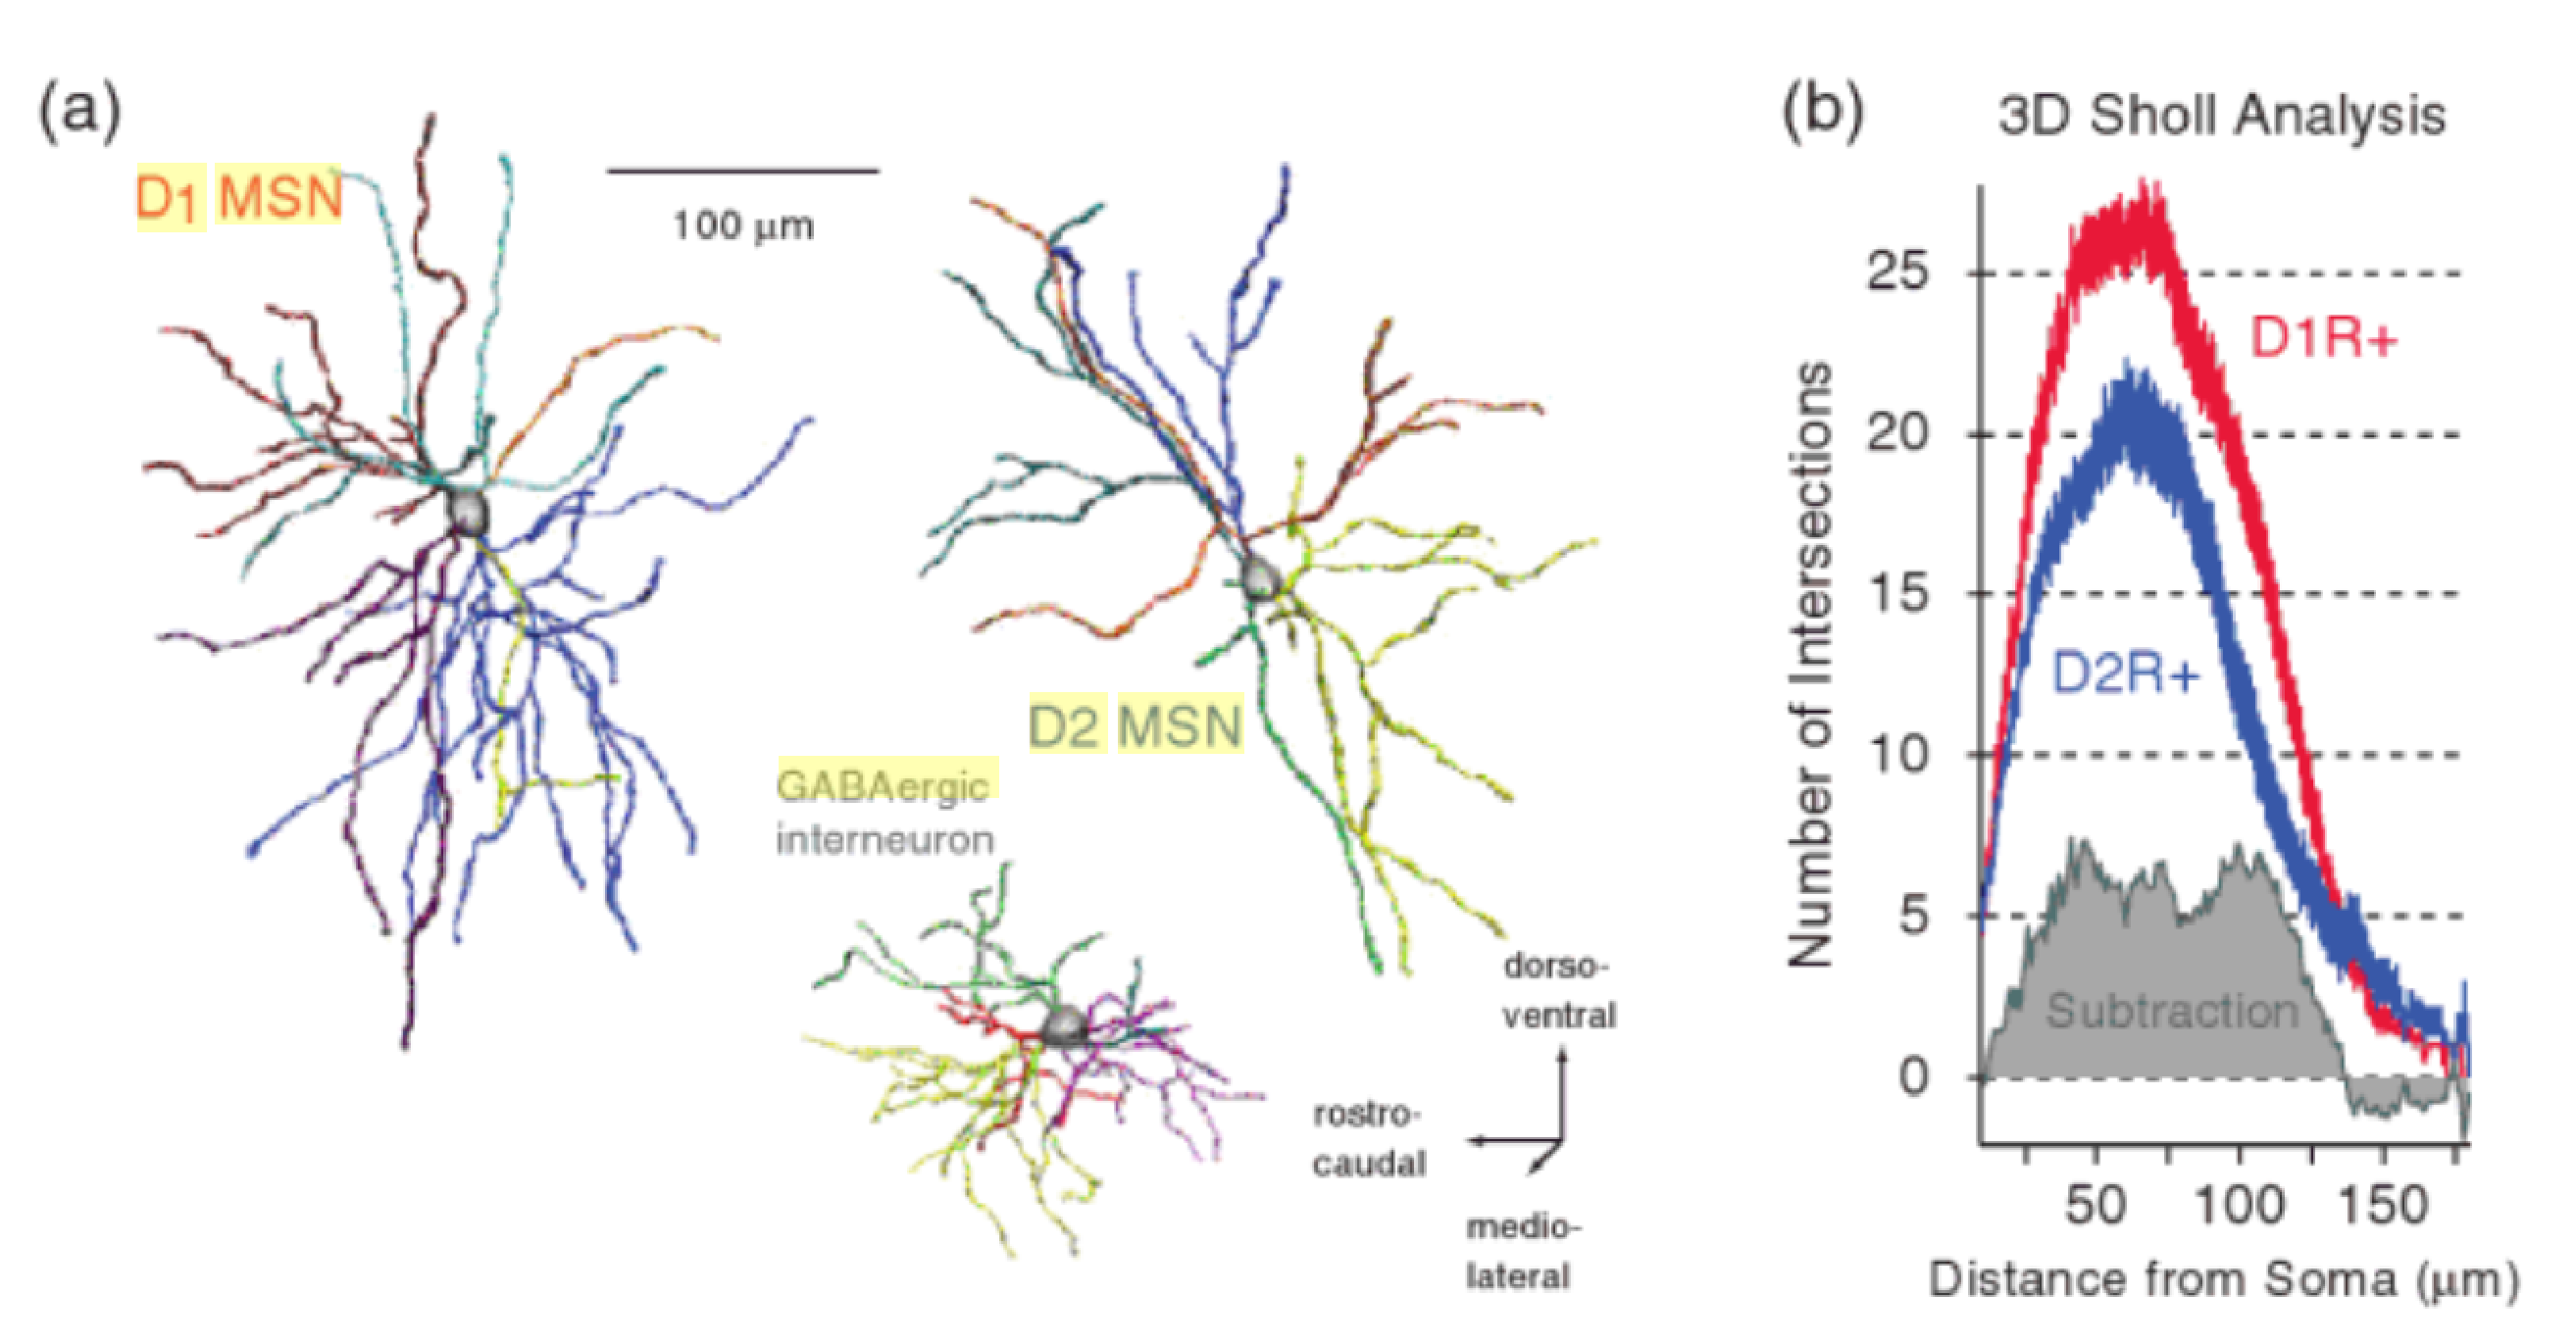
\includegraphics[height=4cm]{./images/MSN-morphology.eps}}
\caption{(A) reconstruction of biocytin-filled D1 and D2 MSN in P35-P45
transgenic mice; (B) 3D Scholl analysis  showing number of intersections at
1$\mum$ eccentricities from the soma for 15 D1+ MSN and 16 D2+ MSN
\citep{bjorklund2010}(pg. 151)}
\label{fig:MSN-morphology}
\end{figure}

Shen et al. (2003) showed mean whole cell capacitance is 7.6$\pm$0.2 pF from 38
MSNs. Assuming $\Csc=1 \mu$F/cm$^2$, then the surface area is 760 $\pm$20
cm$^2$.

Acutely dissociated neostriatal neurons generally have either medium
($\approx$ 10 $\mum$) or large ( $>$20 $\mum$) somal diameters; with
whole-cell capacitance between 2.5 to 10.8 pF (i.e. mean 6.5$\pm 1.7 pF$)
(Nisenbaum et al., 1996).

\subsection{excitability: level of GABAergic projection }

D1+ MSNs exhibit a greater GABAergic inhibitory tonic current than D2+ MSNs in
young mice. Thus, D2+ MSN is more excitable than D1+ MSN,
Fig.\ref{fig:MSN-electrophysiology}

\begin{figure}[hbt]
 \centerline{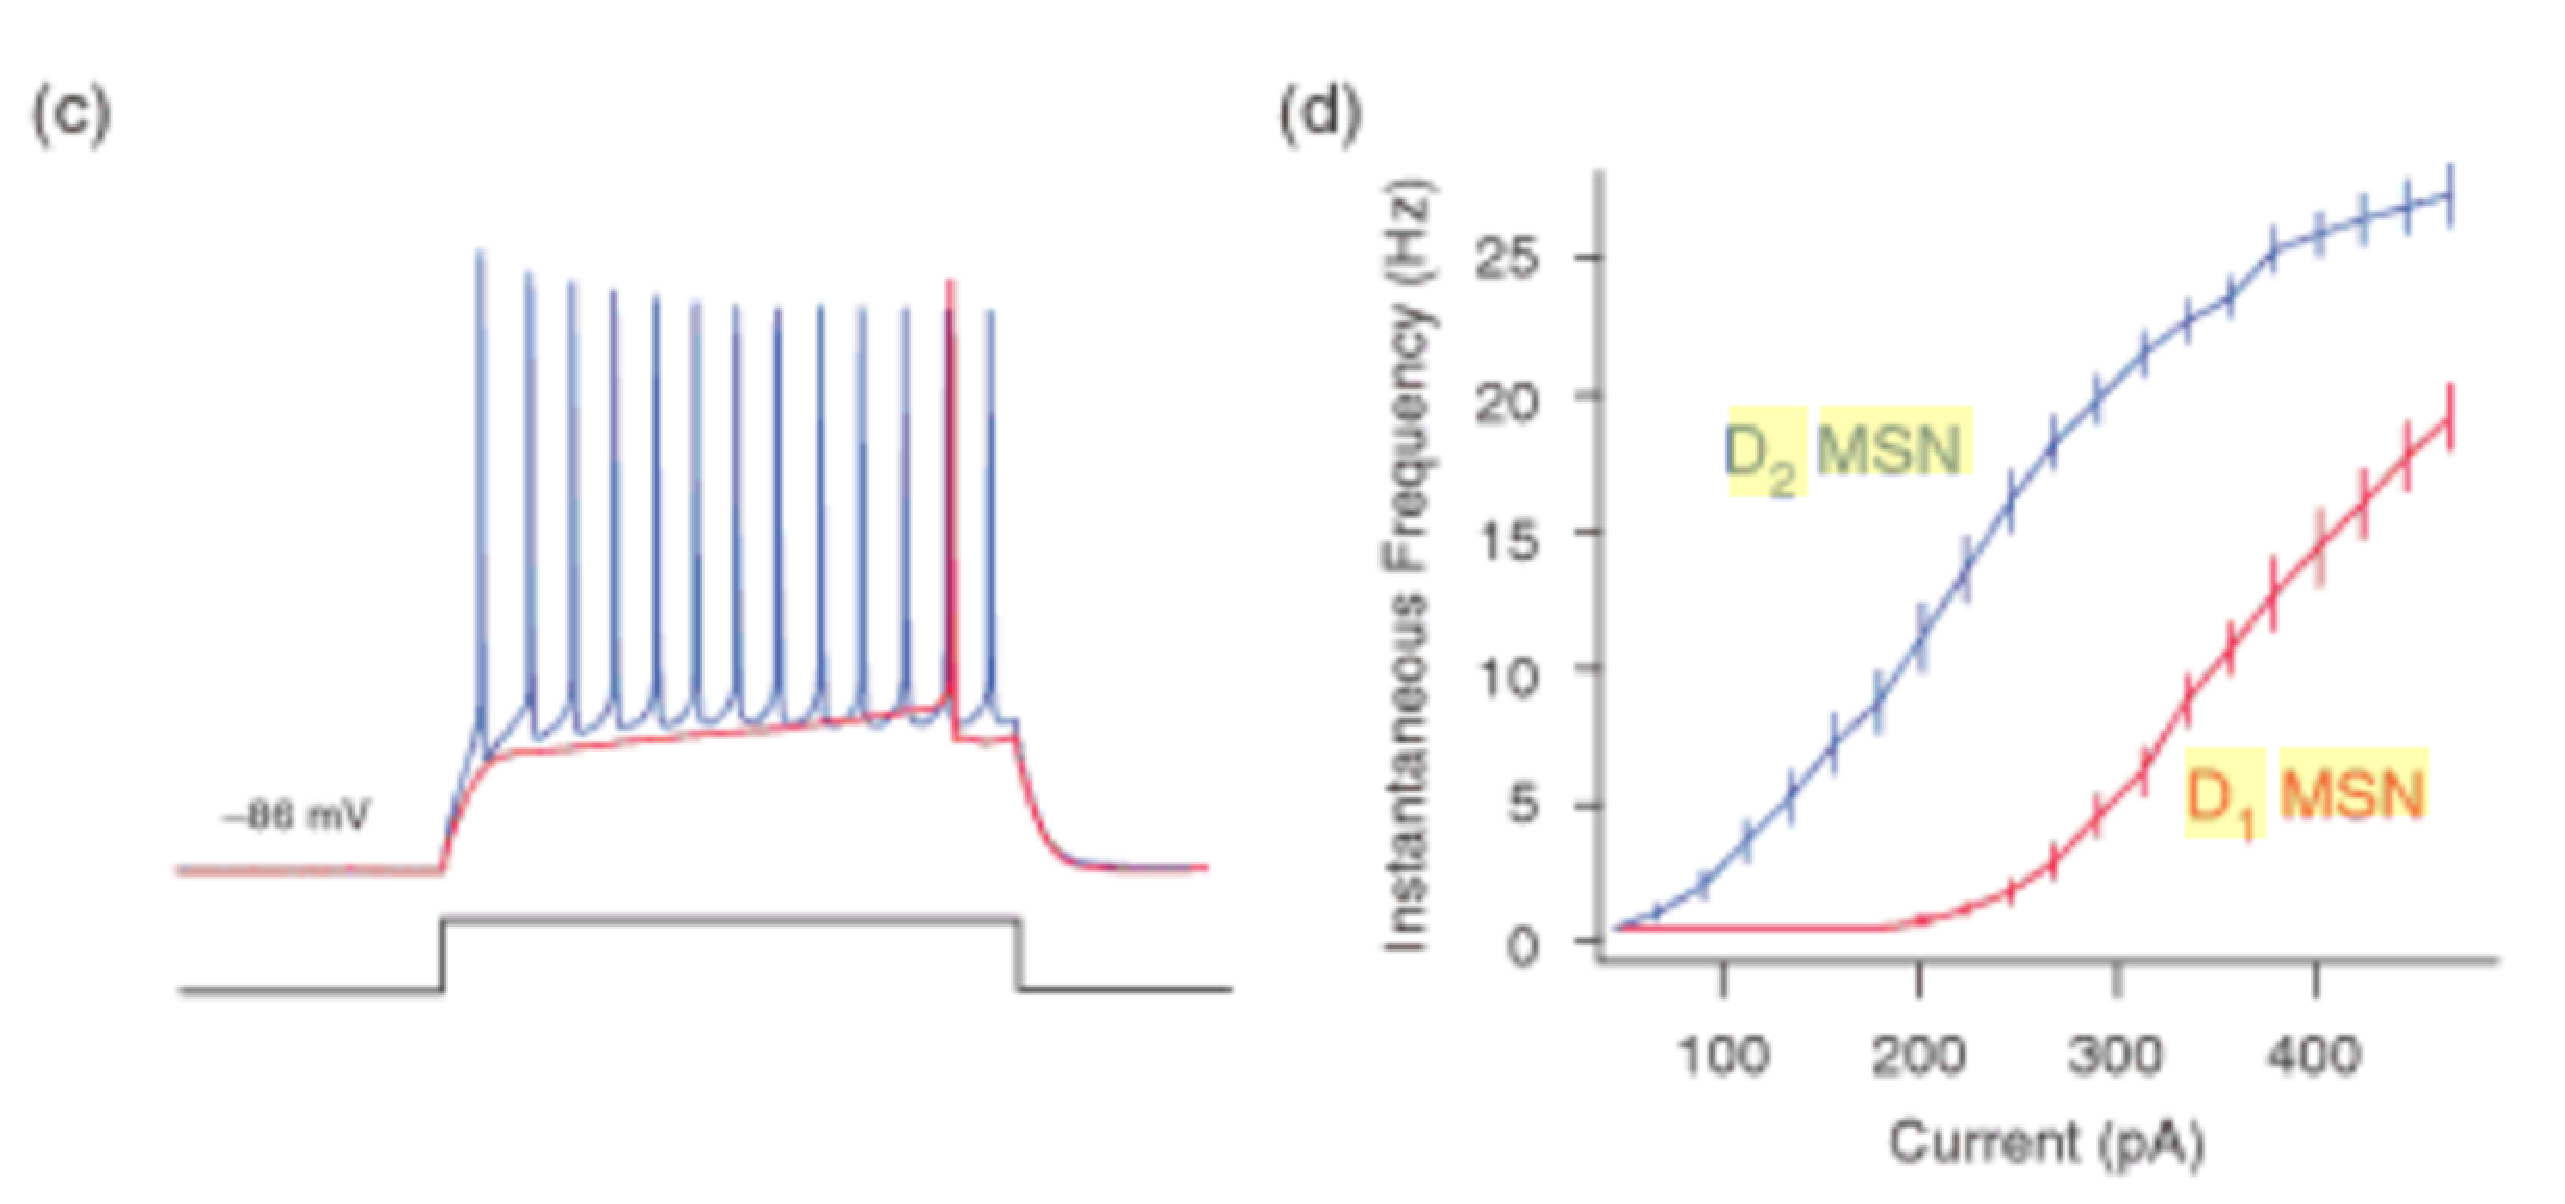
\includegraphics[height=4cm]{./images/MSN-excitability.eps}}
\caption{(C) Membrane response to intra-somatic current injection. (D) at
different amplitude of current injection vs. the firing frequency in D2+ MSN
and D1+ MSN \citep{bjorklund2010}(pg. 151)}
\label{fig:MSN-electrophysiology}
\end{figure}


\subsection{bAP propagation}

The somatic spike in MSN can generate bAP strong enough to depolarize potential
at proximal dendrites and spines (at about 40-50 $\mum$ from soma) to the level
that can open Vm-dependent $\Ca$ channels (Carter and Sabatini, 2004).

To answer whether backpropagation of action potentials (bAPs) occurs in more
distal dendritic regions and whether bAP invasion of the dendrites differs in D1
and D2 MSNs.
\begin{itemize}
  \item \citep{day2008} suggests that normally, bAPs invade more distal
  dendritic regions of D2 MSNs than D1 MSNs. 
  
This  invasion is controlled not only by voltage-dependent Na+
channels but also by Kv4 K+ channels.
DA and acetylcholine (ACh) potently modulate the bAP-evoked
dendritic Ca2+ transient in D2 MSNs, but not in D1 MSN


  \item 
\end{itemize}

In diseases:
\begin{enumerate}
  \item Parkinson's disease (PD): leads to a rapid and selective loss of
spines and glutamatergic synapses in D1 MSN, but not in D2 MSN (Day et al.,
2006).

REMEMBER: spine loss is the result of LTD caused by retrograde signaling which
requires the depolarization-activated Cav1.3 $\Ca$ channel.

This loss selectively increases spike generation in striatopallidal
MSNs.

  \item 
\end{enumerate}

\section{Experiments}

\subsection{Single neuron extraction}

Striata were dissected from young adult (3-4 wk) Sprague-Dawley rats, and medium
spiny neurons were acutely dissociated using previously described procedure
(Surmeier et al. 1992). After the neurons settled to the bottom of the dish,
they were continuously perfused with a physiological saline, i.e.
(in mM) 140 NaCl, 2 KCl, 2 MgCl2, 1 CaCl2, 23 glucose, and 15 HEPES (pH 7.4, 300
mOsm/l).

\subsection{Slice preparation}

For slice preparation, 250 $\Omega$M coronal striatal slices were made in
an artificial cerebrospinal fluid (ACSF) containing (in mM) 125 NaCl,
2.5 KCl, 2 CaCl2, 1 MgCl2, 1.25 NaH2PO4, 24 NaHCO3, and 10
glucose (pH 7.4 with 5\% CO2, 300 mOsm/l). The slices were then
allowed to recover in ACSF for 1 h before recording

\subsection{Recording}

Whole-cell current-clamp recording is performed on MSN neurons in the (rat)
brain slices. The experiment is done using 
\begin{itemize}
  \item  Axoclamp-2A amplifier (AxonInstruments, Union City, CA)  
  
  \item Axopatch 200 or 
  
  \item Multiclamp 700A amplifier
\end{itemize}
and acquired with Axoscope 8.1 (Axon Instruments)
at a sampling rate of 10 kHz.

\begin{mdframed}
Electrode resistance in the bath was typically 1.5-2.5 M$\Omega$ for recording of acutely isolated
neurons and 3-4 M$\Omega$ for slice recording.

Series resistance (7-12 M$\Omega$ in dissociated cells and 10-20 M$\Omega$ in slices) was
compensated (70-90\%) and periodically monitored.
\end{mdframed}

The I-V curve was obtained by injection of 500 ms current pulses (-250 to +250
pA) every 10 s into the neurons on pre-synaptic side.
Suprathreshold depolarizing current pulses were applied and adjusted
to evoke up to five action potentials on the recorded cell.

\section{Older models}

(Wilson, 1995;Wood et al., 2004).

%  Mahon et al., 2000; Kitano et al., 2002;
% Gruber et al., 2003; 

\section{One-compartment models}

(Mahon et al., 2000b; Gruber et al., 2003),

\subsection{Izhikevich (2007)}
\label{sec:Izhikevich-2007-MSN}

\begin{equation}
\begin{split}
\Cm \frac{dV}{dt}= k(V - E_r ) (V - V_\thres) - u + I \\
\frac{du}{dt} = a \left[ b(V - E_r) - u \right]
\end{split}
\end{equation}
with reset condition:
\begin{itemize}
  \item If $V \ge V_\peak$ then $V \leftarrow c, u \leftarrow u + d$
\end{itemize}

NOTE: $\Cm $ is total capacitance, $E_r, V_\thres$ are normal resting and
threshold potential, $I$ is current source, and $c$ is reset potential (i.e. the value of
the membrane potential immediately after an action potential is fired).

Parameter $a$ is the time constant - typically of inactivation - of
the dominant ion channel. Parameters $k$ and $b$ are derived from
the I-V curve of the neuron and $d$ is tuned to achieve the desired
rate of spiking output. 

For MSN, the estimated preliminary parameters by Izhikevich (2007) was
$\Cm = 50$ (pF), $E_r = -80$ (mV), $V_\thres = -20$ (mV), $k=1$, $a=0.01$,
$b = -20$, $c=-55$ (mV), $d = 150$ and $V_\peak = 40$ (mV).



\subsection{Humphries-\ldots-Gurney (2009)}
\label{sec:MSN_HumphriesGurney2009}

\citep{humphries2009} extended the canonical spiking model of (Izhikevich, 2007)
- Sect.\ref{sec:Izhikevich-2007-MSN}), which has been employed in some notably
large-scale models (Izhikevich et al., 2004) to account for dopaminergic
modulation.


\subsection{- Models}

They upgraded Izhikevich (2007) formula 
\begin{enumerate}
  \item replace $I$ with synaptic current
models for GABA, AMPA, and NMDA receptors, including
the NMDA receptor blockade by Mg2+ ions.

  \item 
\end{enumerate}



\subsection{- Conclusion}

The model can reproduce (1) long-delayed spike on first AP, (2) pair-pulse
facilitation (Sect.\ref{sec:pair-pulse-ratio}). But the MSN models are not
bistable, with or without dopamine.


\section{Two-compartment models}

(Kitano et al., 2002),

\section{Wolf et al. (2005) - nucleus accumbens (NAcb)}
\label{sec:Wolf-2005-MSN}

Data are based on MSN in NAc (Sect.\ref{sec:nucleus_accumbens}), with some data
extracted from dorsal striatum's MSN (Sect.\ref{sec:dorsal-striatum}).
  
The first model to add all reported $\Ca$ current components, and
$\Ca$-dependent potassium currents.



\subsection{Conclusion}

Tuning: maximal current conductance in each compartment $\rightarrow$ to 
achieve the behavior matching closely whole-cell recording from adult rat NAcb.

The model can
\begin{enumerate}
  \item reproduce long delay at first AP at rheobase
  \item low frequency of spiking
\end{enumerate}

The model was used to test the effects of the NMDA/AMPA ratio on entrainment to
oscillation.

\subsection{Morphology}

A simple stylized morphology of the cell, Fig.\ref{fig:MSN-Wolf}(B), was
developed based on anatomical data in accumbens (O'Donnell and Grace, 1993). It has 4 primary
dendritic branches. Each primary branch bifurcates twice, resulting in 16
tertiary dendrites. Published values of dendritic length and diameter in NAcb
(O'Donnell and Grace, 1993) match those in dorsal striatum (Wilson, 1992).

\begin{figure}[hbt]
  \centerline{
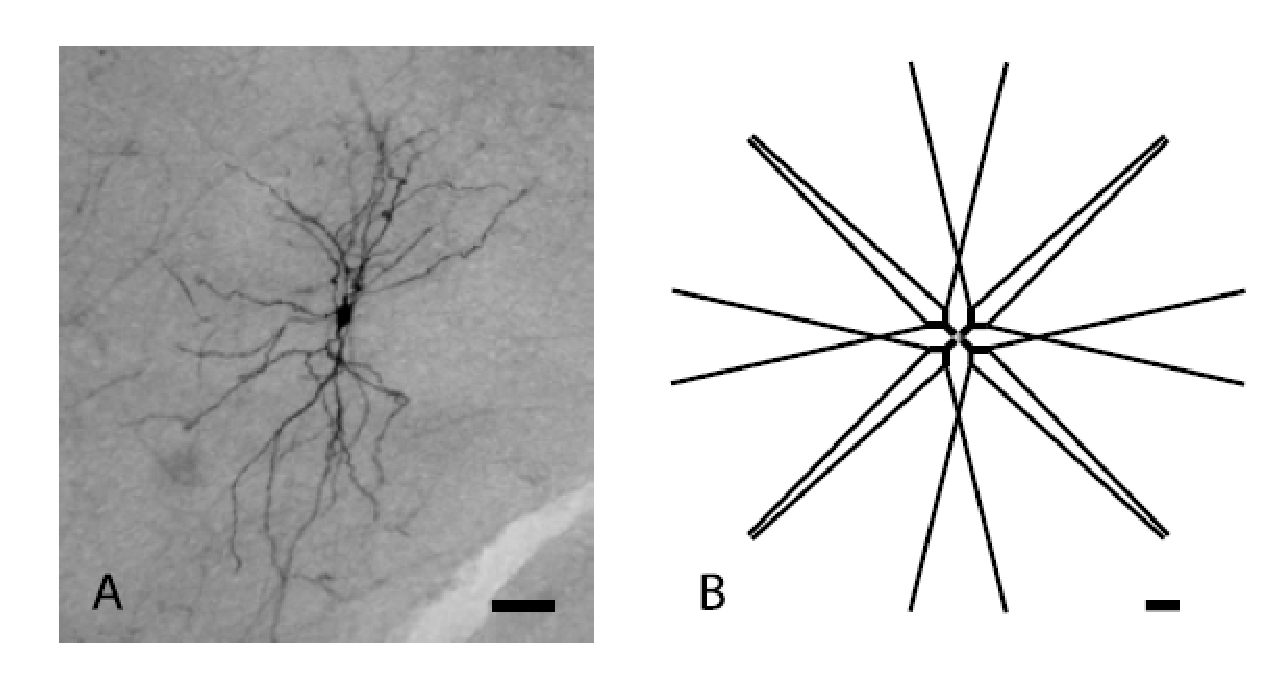
\includegraphics[height=10cm,
    angle=0]{./images/MSN-Wolf2005.eps}
    }
\caption{MSN morphology, and its representation in the model}
\label{fig:MSN-Wolf}
\end{figure}

\begin{itemize}
  \item primary branches: 1 compartment/branch (length 20 $\mum$)
  \item secondary branches: 1 compartment/branch (length 20 $\mum$)
  \item tertiary branches: 11 compartments/branch to ensure spatial accuracy 
  (length 190 $\mum$ total)
\end{itemize}

\subsection{Tuning}

To calibrate model parameters (in this case is maximum conductances),
conductance parameters were tuned so that the response of the model cell matched
that of in vitro MSP cells to both subthreshold and suprathreshold current
injections.

EXPERIMENT: The electrophysiological properties of NAcb MSP cells were examined
under current clamp using whole-cell patch recordings in vitro on NAcb MSP cells
in slices of the young adult rat.
\begin{itemize}
  \item 
\end{itemize}

The parameters include published parameters for accumbens, supplementing
these with dorsal striatal parameters, and finally using measurements
from other neurons when necessary.

Activation and inactivation time constants were temperature corrected to
35$^\circ$C to match electrophysiology recordings.

The leak conductance $g_\leak$ and inwardly rectifying potassium current
conductance was adjusted to get the apparent input resistance of 79.7 M$\Omega$
of our in vitro cell.

\subsection{Model}



Model
\begin{itemize}
  
  \item  include all known intrinsic channel components (so far)
  
  \item synaptic input of spines: 2 types of synapses (1) NMDA, AMPA; 
  (2) GABA-A receptors.
  
  \item 
\end{itemize}

Standard value: (Gentet et al., 2001)
\begin{itemize}
  \item axial resistance $R_a = 100 \Omega/\cm$ = 
  
  \item $\Csc = 1.0 \muF/\cm^2$
\end{itemize} 

{\bf Leak}: $g_\leak = 11.5 \muS/\cm^2$, $E_\leak = -70$ (mV).

\subsection{- Channels}

Channels
\begin{enumerate}
  \item  fast (NaF, NaT) - Sect.\ref{sec:NaT-Wolf-2005} and 
  
  
  \item persistent sodium (NaP) - Sect.\ref{sec:NaP-Wolf-2005}

NOTE: They claimed that uniform distribution of sodium current leads to
unrealistic behavior; i.e. they set total conductance of sodium in the soma was
set to be 10 times the total conductance of sodium in the dendrites

  
  \item fast-inactivating (KAf) and 
  \item slow-inactivating (KAs) A-type,
  
  \item 4-aminopyridine (4-AP)-resistant, persistent delayed-rectifying (KRP), and 
  
  \item inward-rectifying (KIR) potassium currents; 
  
  \item large-conductance (BK) and 
  \item small-conductance (SK) calcium-dependent
  potassium currents; 
  
  \item N- (CaN), P/Q- (CaP/Q), R- (CaR), and L-type (Cav1.2) highvoltage-
activated calcium channels; and 
  \item T- (CaT) and L-type (Cav1.3) low-voltage-activated calcium channels
\end{enumerate}
These channels
were distributed throughout the cell in accordance with published data
when possible. If not known, channels were assumed to be distributed
uniformly throughout the cell unless this resulted in nonphysiological
behavior.

\subsection{- [Ca] internal}

The internal calcium in a thin shell just under the cell membrane, but not
the whole myoplasm, is tracked for every compartment. 

Calcium influx was balanced against diffusion and pumping activity to provide
appropriate calcium sensitivity for both SK and BK KCa channels.

Two different Calcium pools is used:
Experimental data has indicated that striatal calcium-dependent potassium
channels are activated by calcium influx through N- and Q-type calcium channels
but not L-types (Vilchis et al., 2000). Accordingly, we specify a calcium pool
for 1.2 and 1.3 L-type currents and a separate calcium pool for N-, Q-, and R-
type calcium currents with which the calcium-dependent potassium channels are
associated.

\subsection{- Receptors: NMDA, AMPA, GABA}

NMDA, AMPA, and GABA currents were modeled
using a modified two-state synapse (based on the Exp2Syn synapse in NEURON)

\subsection{- implicit spines}

With the length for each compartment, it is assumed that there are spines on all
of these compartments. As the spines are not treated explicitly, the 
surface area for each compartment need to be adjusted to compensate for
additional membrane area attributable to spines using these equations
\begin{equation}
\begin{split}
l' = l \times F^{2/3} \\
d' = d \times F^{1/3} \\
F = \frac{A_{dend} + A_{spine}}{A_{dend}}
\end{split}
\end{equation}
The formula for F is based on Segev-Burke (1998).

The surface area parameters $A_{dend}$ and $A_{spine}$ were based on published
values of spine density in striatal MSP cells (Wilson, 1992).



\subsection{Numerical method}

\begin{enumerate}
  \item use NEURON software: 189 compartments
  
  NEURON tools is used (running on 12-node cluster): 189-compartment model.
\verb!d_lambda=0.15! is chosen in NEURON software so that each compartment of
length 20$\mum$.

  \item Apple Computers (Cupertino, CA) dual 2.5 GHz Power Macintosh G5 or in
  parallel on a 12-node cluster with dual 2.8 GHz processors per node (Penguin
  Computing, San  Francisco, CA).
\end{enumerate}


Inputs were placed in the middle of the appropriate compartment to
acquire second-order correct solutions.

\section{Moyer (2007) - dopamine}
\label{sec:MSN_Moyer2007}

Dopaminergic modulation produces a variety of functional changes in the principal cell of the
striatum, the medium spiny neuron (MSN). 

The effects of DA on the MSN have been extensively studied and depend on the
class of receptor expressed by the cell. Most MSNs coexpress two or more species
of receptors, although D1 and D2 receptors (D1R and D2R, respectively) are the
most prevalent.

They tested 2 hypothesis:

\begin{enumerate}

  \item D1R-mediated modulation increases the nonlinearity
of MSN cell output in response to synaptic input (Gruber et al. 2003;
Hernandez-Lopez et al. 1997; Nicola et al. 2000).

It is based on the observation that MSN cells in in vivo anesthetized
preparations oscillate between a hyperpolarized membrane potential (down-state)
and a depolarized plateau potential in which the cell may generate action
potentials (up-state) (Goto and O'Donnell 2001; Stern et al. 1997; Tseng et al.
2001; Wickens and Wilson 1998; Wilson and Kawaguchi 1996).

{\it DA-enhanced nonlinearity} would increase the tendency for the cell to dwell
in one of these two states, potentially contributing to gating (O'Donnell and Grace
1995), pattern recognition (Houk 1995), or credit assignment (Kerr and Plenz
2002, 2004) at the network level.

{\it DA activation of D1Rs increases striatal output, whereas D2R activation
reduces striatal output} (Albin et al. 1989; Bamford et al. 2004; Cepeda and
Levine 1998; Delong 1990; Gonon 1997; Goto and Grace 2005b)

DA regulates the balance of the direct, D1R-expressing, movement-facilitatory
pathway and the indirect, D2R-expressing, movement-inhibitory pathway (Albin et
al. 1989; Delong 1990).

loss of DA innervation to the striatum, as in Parkinson's disease, biases
control of the basal ganglia output toward the movementinhibiting
indirect pathway, resulting in deficits in movement
initiation and execution
 
DA acts as an input filtering mechanism,
suppressing weak inputs while permitting or even enhancing
stronger inputs (Cepeda and Levine 1998; Hjelmstad 2004;
Nicola et al. 2000, 2004). This could enhance the signal-tonoise
ratio of MSN inputs.

  \item dopamine might affect the integration time
window of the MSN.

DA could alter the integrative behavior of striatal cells, shifting their
behavior in the direction of either integration or coincidence detection.

Such an effect could presumably modulate the overall integration of inputs in
the corticostriatal network, which may affect the behavioral output of the
system.
\end{enumerate}

D1 modulation decreases the SK current (by CaN and CaQ reduction)
and increases the Cav1.3 calcium current. 

\subsection{Conclusion}

The model was used to test the effects of dopamine modulation on synaptic
integration.

We found that dopaminergic modulation had no effect on nonlinearity or
bistability of the MSN, except at very high, apparently nonphysiological levels
of NMDA conductance.

DA modulation was able to regulate neuronal excitability and input filtering in
the MSN and was also capable of modulating the temporal integrative properties
of the MSN. In these cases, the synaptic effects of DA modulation counteracted
and overcame the intrinsic effects of DA modulation

\subsection{Model}

This is an extension to the 189-compartment model of Wolf et al. (2005) -
Sect.\ref{sec:Wolf-2005-MSN}. They created a new version of the
model 
\begin{enumerate}
  \item High-calcium model: to support $\Ca$
spiking: with approximately 10x higher calcium channel expression
for all classes of calcium than that of the ``low-calcium'' version presented
previously

NOTE: at least some striatal cells exhibit calcium spiking after 4-aminopyridine
(4-AP) and tetrodotoxin (TTX) application (O'Donnell and Grace 1993), which
was not supported in the previous model. \textcolor{red}{The authors assumed
the spike is caused by higher $\Ca$ expression}


  \item SK current: only present in secondary and tertiary dendrites only.
  in agreement with studies suggesting that SK channels are expressed
primarily in dendritic spines (Faber et al. 2005; Ngo-Anh et al. 2005;
Obermair et al. 2003).

  
  original (uniform throughout the cell) 
  
  \item a rapidly activating, delayed rectifier
Kv1.3 (KDR) current was added at uniform conductance throughout the cell -
Sect.\ref{sec:delay-rectifier}. The KDR channel was inserted at a uniform
conductance of $5.0 \times 10^{-4}$ S/cm2 throughout the cell.

NOTE: Modulations of DA can enhance the tendency of the model to spike in
doublets. At the extreme modulation levels that we study here
we occasionally observed doublets at high-input levels. 
\textcolor{red}{Kv1.3 was added to address this}.
It is similar
to the KRP current (Nisenbaum et al. 1996) in that it is a
tetraethylammonium (TEA)-sensitive, delayed-rectifier current.
However, it activates about fivefold faster and at more hyperpolarized
potentials, allowing it to suppress doublets without significantly
affecting subthreshold activity.

Kv1.3 is used because it has been well characterized in a computational model
(Erisir et al. 1999) and behaves similarly to the Kv1.1 and Kv1.6 channels
(Coetzee et al. 1999), which have been detected in MSN cells using mRNA assays
(Shen et al. 2004).
Kv1.3 channel is used as a substitute for the Kv1.1/1.6 channels and suggest
that these currents may represent a portion of the TEAsensitive,
delayed-rectifier current in MSNs.
  
  \item the cell was retuned after these changes to match in
vitro current-clamp data, including spike shape, frequency response, and
subthreshold membrane response of a nucleus accumbens core cell.

This included changing the maximum conductance of many channels and implementing
a -2 mV shift of the fast sodium channel Naf.

\end{enumerate}

\subsection{Synapses: glutamatergic + GABAergic}

Each NMDA/AMPAR synapse or GABA synapse is a modified two-state synapse with
time constants set to published values (Chapman et al. 2003; Galarreta and
Hestrin 1997; Gotz et al. 1997).

The ratio of glutamatergic inputs to GABA inputs was held constant at roughly
1:1 for all simulations (Blackwell et al. 2003).

Synaptic inputs were modeled using a modified version of the NetStim object
provided in the NEURON package.
Each synapse (AMPA/NMDA or GABA) received an independent spike train generated
using MATLAB. Each spike train was generated using the
following algorithm
\begin{enumerate}
  \item a constant interspike interval (ISI) train was
generated at the desired frequency
  \item then pulled a new from a Gaussian distribution centered at the original
  spike time
\end{enumerate}
The resulting train was then randomly shifted; this process was repeated
for each of the 168 total synapses. Input was generated by using a
large shift (one ISI) and a large SD (1/4 of the ISI).


\subsection{- Glutamatergic}

Each glutamatergic synapse consisted of an AMPA and NMDA pair receiving the same
input train. AMPA and NMDA channels contributed to the calcium pool
not associated with the SK/BK currents: 10\% of NMDA current and
0.5\% of AMPA current were designated as calcium currents as
described in previous studies (Burnashev et al. 1995).

They are placed throughout the dendrites, in accordance with published
results (Gracy et al. 1999; Wilson 1992).

\subsection{- GABAergic}

GABAergic synapses were distributed throughout the cell but {\it clustered near
the soma} in agreement with physiological data (Fujiyama et al. 2000; Pickel and
Heras 1996).

$\gamma$-aminobutyric acid (GABA) (Nusser et al. 1998) conductance levels were
set to published value.

\subsection{Tuning}

The model was tuned by hand

\section{Steephen-Machanda (2009)}
\label{sec:Steephen-Machanda-2009-MSN}

This model adapted the works of Wolf et al. and Moyer et al.. The inwardly
rectifying potassium current (Kir) was re-tuned, to investigate the role of
inactivating Kir in MSN excitability.

\section{Spiga et al. (2010)}

Also adapted the works of Wolf et al and Moyer et al., they added morphology
based on a digital reconstruction of an MSN and tested the effects of spine loss
and AMPA current reduction on AP frequency during simulated upstates.

\section{Gertler et al. (2008)}
\label{sec:Gertler-2008}

\subsection{Model}

\begin{enumerate}
  \item 1 Na+ current
  
  \item 1 Ca2+ current
  
  \item 5 K+ currents
  
  \item AMPA
\end{enumerate}

The model was used to test the contribution of morphological differences between
D1 and D2 MSNs in describing their different electrophysiological characteristics

\section{Day et al. 2008}

A similar model to Sect.\ref{sec:Gertler-2008} investigate the back propagation
of the action potential into MSN dendrites.

\section{Plotkin et al. (2011)}

They adopted Sect.\ref{sec:Gertler-2008}	

\section{Flores-Barrera (2009)}

\begin{enumerate}
  \item 1 Na+ current
  
  \item 2 Ca2+ current
  
  \item 5 K+ currents
  
  \item AMPA, NMDA, GABA
\end{enumerate}

This model is used to test whether GABAergic input, which is depolarizing below
its reversal potential (roughly -60mV), plays a role in maintaining the
depolarization of an MSN during a cortico-striatal upstate.

\section{Evans et al. (2013)}
\label{sec:Evans-2012}

\citep{evans2012} proposed a dorsal striatum MSPN model by modifying that of
Wolf (2005) (Sect.\ref{sec:Wolf-2005-MSN}) for mature (> 3 weeks old) mouse dorsal
striatum.
\begin{itemize}
  \item morphology is the same
  
  \item update: channel concentration + kinetics
\end{itemize}

\subsection{Model}

\begin{enumerate}
  \item 1 Na+ current
  
  \item 5 Ca2+ current
  
  \item 6 K+ currents
  
  \item 4 different types of AMPA, NMDA. 
  
  \item 1 GABA
\end{enumerate}

This model is used to test whether the NMDA receptor subtypes, based on the four
GluN2 subunits, differentially affect the calcium influx into spines during
closely-timed pairings of pre and post-synaptic activity (spike timing dependent
plasticity protocols).


\section{Nakano et al. (2013) - add ER calcium release via IP3R + RYR}

The calcium release from ER through IP3R and RyR is suggested to significantly
affect the activity of various neurons (Falcke et al.,2000; Varona et
al.,2001b,a).

They added $[\Ca]_\ER$, but only for the spines, not for the dendrites.


\subsection{Conclusion}

\subsection{Model}

A 156 compartment neuron model is developed based on their 3D reconstructed
morphology MSN, with model components are based on previous works
(Sect.\ref{sec:Wolf-2005-MSN}, \ref{sec:MSN_Moyer2007}).
\begin{itemize}
  \item 2 $\na$ current components
  \item 6 $\K$ current components
  \item 6 $\Ca$ current components
\end{itemize}

To emulate the modulation of DA, each channel is multiplied with a coefficient
$\mu_i$, with $i$ represents the proper ion channel. 

\begin{equation}
\begin{split}
I_\text{Na} = \mu_{NaF} I_{NaF} + \mu_{NaP} I_{NaP} \\
I_\text{K} = \mu_{KAs} I_{KAs} +
    \mu_{KAf} I_{KAf}  + \mu_{KRP} I_{KRP} + \mu_{KIR} I_{KIR} + \mu_{SK} I_{SK}
    + \mu_{BK} I_{BK} \\
I_\text{Ca} = \mu_{CaN} I_{CaN} + \mu_{CaPQ} I_{CaPQ} +
       \mu_{CaR} I_{CaR} + \mu_{Cav1.2} I_{Cav1.2} +
       \mu_{CaT} I_{CaT} + \mu_{Cav1.3} I_{Cav1.3} \\
I_\syn = \mu_{AMPA} I_{AMPA} + \mu_{NMDA} I_{NMDA}
\end{split}
\end{equation}
If $\mu_i = 0$, it means there is no DA modulation effect on channel of
ion $i$-th.


Still there is no explicit spines are added, so the length (i.e. the leak
conductance) and capacitance has to be adjusted based on the previous model
(Sect.\ref{sec:MSN_Moyer2007}).

\begin{equation}
\begin{split}
F_j = \frac{A_{dend,j} + A_{spine,j}}{A_{dend,j}} \\
g'_{\leak,j} = g_{\leak,j} \times F_j \\
C'_j = C_j \times F_j \\
\end{split}
\end{equation}

All channels in Hodgkin-Huxley form have the same dynamics (activation,
inactivation); the only difference was the maximum
conductance $\bar{g_i}$ and maximum permeability $\bar{p_i}$, to
fit the experimental data using Neurofitter (Geit
et al.,2007).

\subsection{- Hodgkin-Huxley-type}

The current through each type z of $\K$ and $\Na$ channel, was given
by the Hodgkin-Huxley type equations

The current through each type z of NMDA and AMPA receptor, was given
by the Hodgkin-Huxley type equations. 



\subsection{- GHK-type}

The current through each type z of $\Ca$ channel, was given
by the Goldman-Hodgkin-Katz (GHK) current formulation (Sect.\ref{sec:GHK_current})

\subsection{- Calcium release from ER}

It is modeled based on De Schutter and Smolen (1998).

\begin{equation}
\begin{split}
\frac{d[\Ca]_i}{dt } = J_{RYR} + I_{IP3R} - J_\SERCA
           + J_\leak + J_\text{Ca current} - J_\PMCA
           + \left( [\Ca]_{i,\infty} - [\Ca]_i \right) / \tau \\
J_\text{Ca current} = - \frac{I_{Ca} + c_{AMPA} I_{AMPA} + c{NMDA} I_{NMDA}}{2F
V}
\end{split}           
\end{equation}
with $V = $volume of the compartment (i.e. the spine)


\subsection{Analysis}

To measure $\Ca$ transient in spikes, two spines of diameter 1$\mum$ and length
1.273 $\mum$ (volume: 1$\mum^3$) were attached to 2 locations: proximal and
distal dendrites, at 25$mum$ and 100$\mum$ away from soma.

\section{Tuan et al. (2016) - }

\begin{enumerate}
  \item The spine is modeled with the spine neck and the spine head 
  
  (before): treated as one compartment
  
  \item The spines are treated explicitly, with about 10,000 spines per MSN

  (before): ignore it, and substitute the change in membrane surface area
  for the branch
  
  \item  The $[\Ca]_\ER$ is now extended not only on the spines, but also every
dendrites.
  
  \item Update $[\Ca]_o$ to use physiological range: 1.8mM
  
  \item Role of DA is updated, i.e. not using a simple coefficient factor.
\end{enumerate}

\subsection{Model}

\begin{enumerate}
  \item 
  
  \item SK current: only present on spines head + neck
\begin{verbatim}
BRANCHTYPE MTYPE
?  ?  [SK] 
\end{verbatim}
  
  in agreement with studies suggesting that SK channels are expressed
primarily in dendritic spines (Faber et al. 2005; Ngo-Anh et al. 2005;
Obermair et al. 2003).


\end{enumerate}